\begin{figure}[htbp]
  \centering
  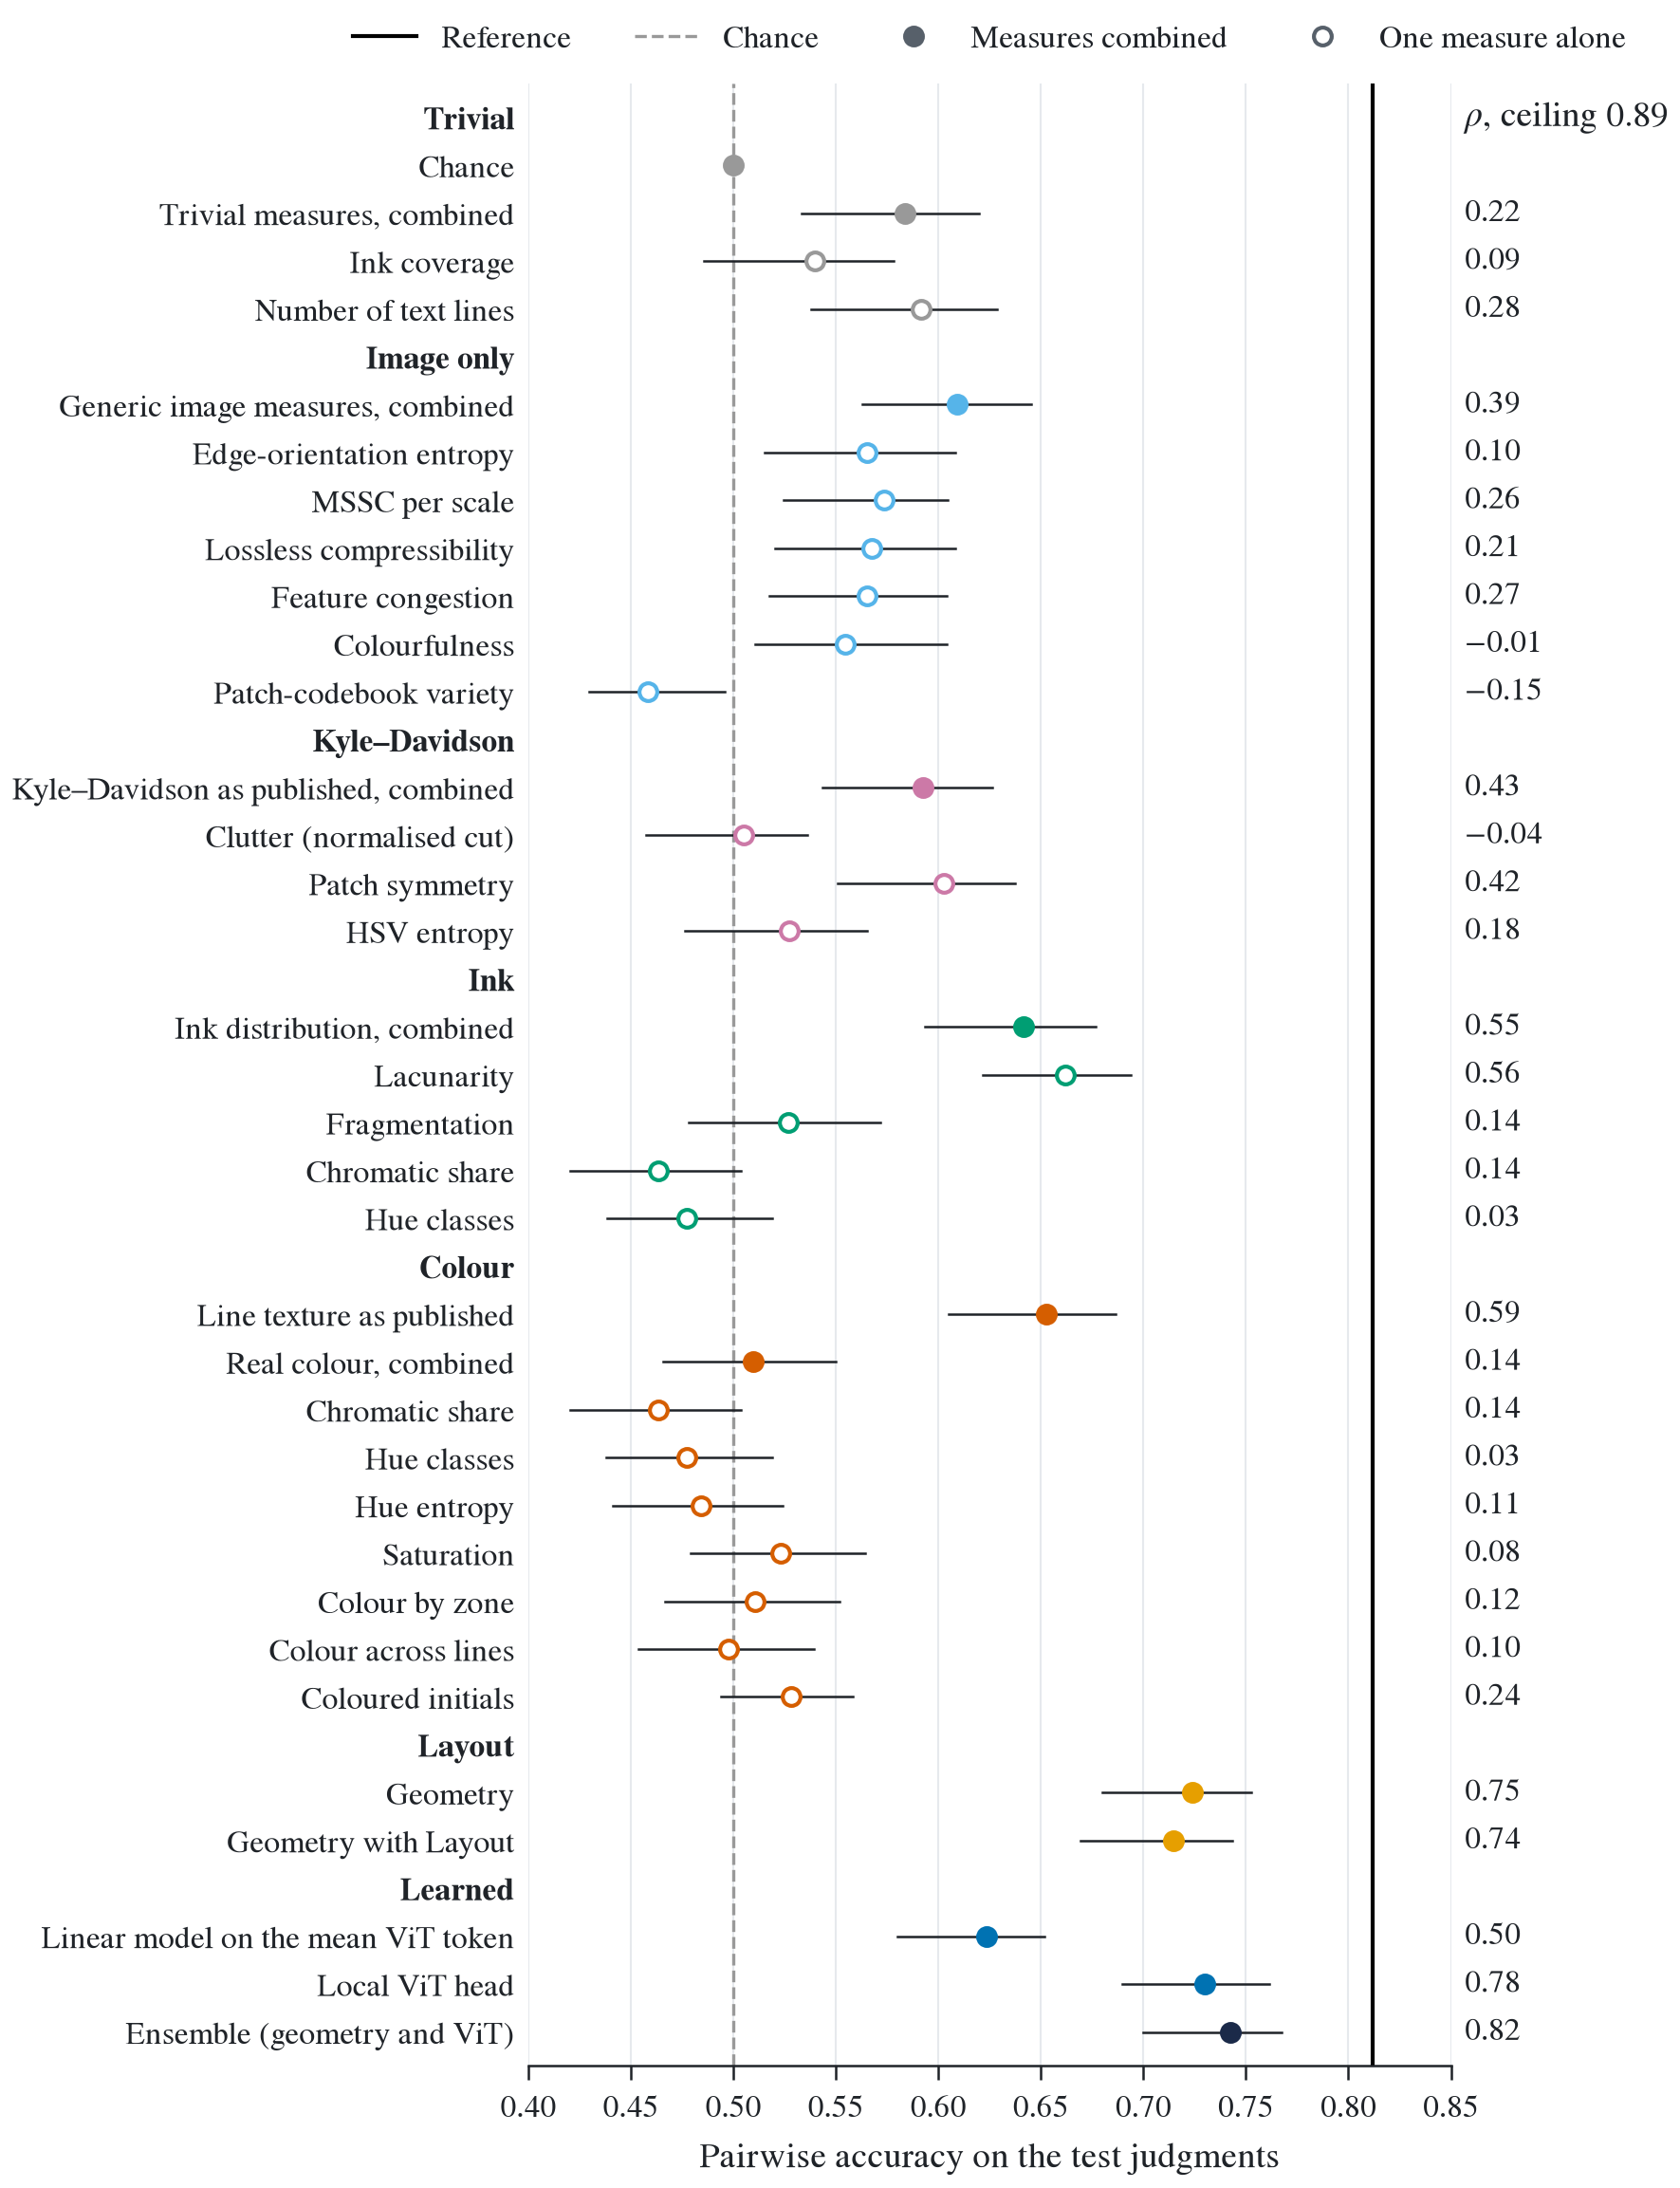
\includegraphics[width=15.00cm]{figures/baselines_by_information_each_measure.png}
  \caption{What each level of information buys: pairwise accuracy on the test judgments (dots, the mean over the folds, with 95\% intervals from 1,000 resamples of the manuscripts) and Spearman's $\rho$ between the out-of-fold page scores and the Elo scores (right), the methods grouped by the information they need (trivial, image only, kyle--davidson, ink, colour, layout, learned). Filled dots: measures combined in one model; open dots: one measure alone, the pairwise logistic model on that measure's columns (the measures are defined in Table~\ref{tab:baseline_measures}). The solid line is the Reference for accuracy (0.812), the consistency of the same test judgments with the final Elo scores (the share that agree with them); the Reference for $\rho$ is its ceiling (0.891), the square root of the Elo scores' reliability: one limit, measured for accuracy and for $\rho$. The dashed line is chance. \emph{Trivial measures, combined}, the pairwise logistic model on the two trivial measures, ink coverage and number of text lines (2 columns); \emph{Generic image measures, combined}, the pairwise logistic model on the six generic image measures, edge-orientation entropy, MSSC, lossless compressibility, feature congestion, colourfulness and patch-codebook variety (15 columns); \emph{Kyle--Davidson as published, combined}, the pairwise logistic model on the three Kyle--Davidson measures, clutter, symmetry and entropy (7 columns); \emph{Ink distribution, combined}, the pairwise logistic model on the five ink distribution measures, coverage, lacunarity, fragmentation, chromatic share and hue classes (12 columns); \emph{Line texture as published}, the pairwise logistic model on the 38 line-texture features; \emph{Real colour, combined}, the pairwise logistic model on the seven real colour measures, chromatic share, hue classes, hue entropy, saturation, colour by zone, colour across lines and coloured initials (17 columns); \emph{Geometry}, the pairwise logistic model on the 83 geometric features; \emph{Geometry with Layout}, the pairwise logistic model on the 105 geometric and Layout features; \emph{Linear model on the mean ViT token}, the pairwise logistic model on the mean of the page's patch tokens (384 dimensions); \emph{Local ViT head}, the local scoring head on the patch tokens of DINOv2 ViT-S/14 (block 12, 518 pixels on the long edge, the folio crop): an MLP (384--128--1, ReLU, softplus) scoring each patch, the page's score the mean of its patches', trained with RankNet's logistic loss (180 epochs of Adam); \emph{Ensemble (geometry and ViT)}, the mean of the z-scored page scores of \emph{Geometry} and \emph{Local ViT head}. Each method is evaluated by 10-fold cross-validation repeated 10 times, each manuscript's pages in one fold; a fold tests the judgments between two of its pages.}
  \label{fig:baselines_by_information_each_measure}
\end{figure}
